\begin{figure}[h!]
    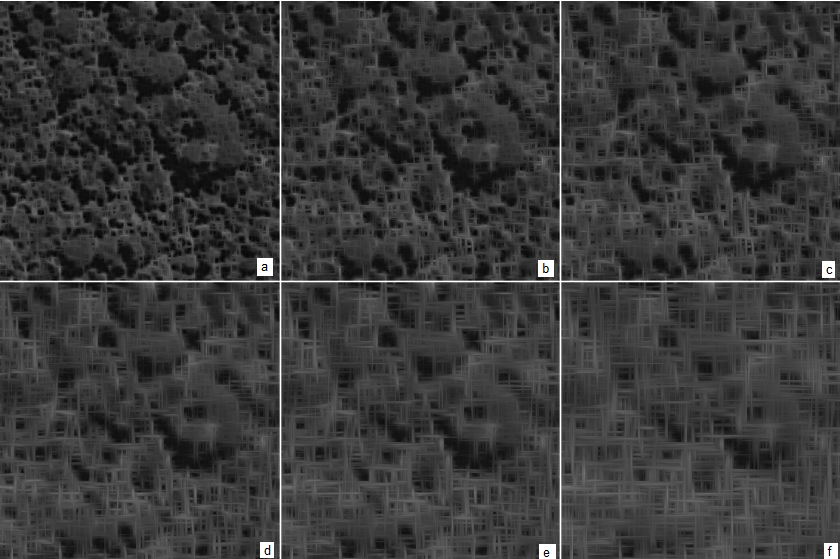
\includegraphics[width=\textwidth]{Imagenes/Resultados script morfologico/GS04-labeled.png}
     %\hfill
     \caption{Resultado del algoritmo Rollingball para tamaños de ventana de a) 6, b) 9, c) 12, d) 15, e) 18 y f) 24 píxeles}
    \label{Rollingball}
\end{figure}
%-------------------------------------------------------------------------------------------------------
\begin{figure}[h!]
    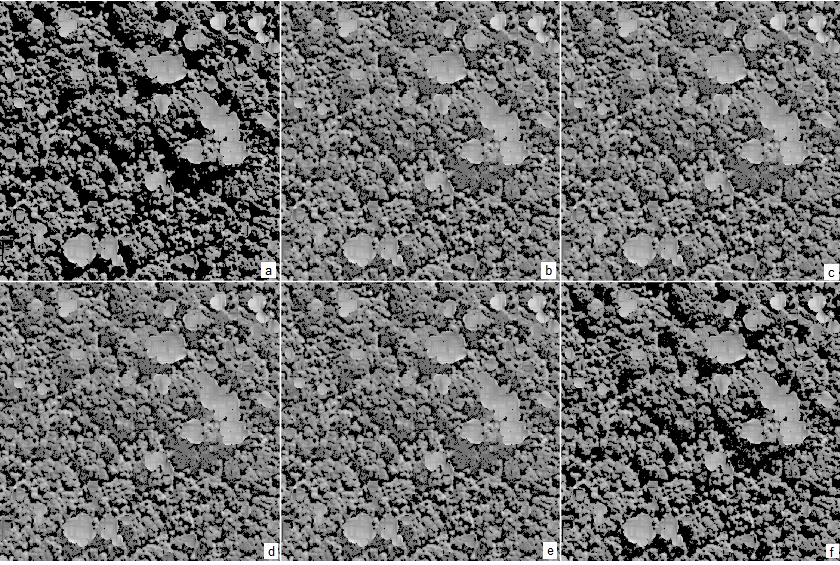
\includegraphics[width=\textwidth]{Imagenes/Resultados script morfologico/GS06-labeled.png}
     %\hfill
     \caption{Resultado de la segunda selección de objetos oscuros con distintos valores de percentil, a) 99, b) 0,1, c) 1, d) 10, e) 50 y f) 90 }
    \label{segundaoscuros}
\end{figure}
%-------------------------------------------------------------------------------------------------------
\begin{figure}[h!]
    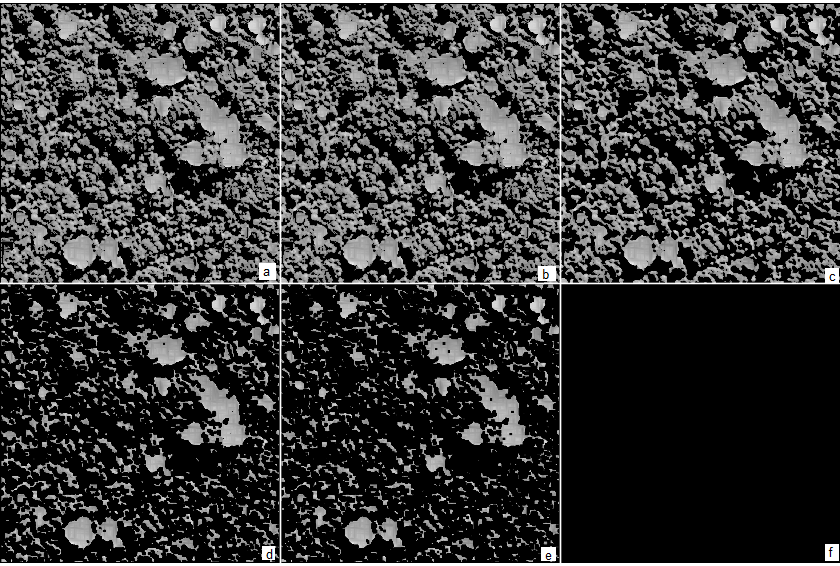
\includegraphics[width=\textwidth]{Imagenes/Resultados script morfologico/GS07-labeled.png}
     %\hfill
     \caption{Resultado de la búsqueda de pequeños huecos con distintos valores de percentil, a) 10, b) 30, c) 50, d) 75, e) 80 y f) 90 }
    \label{pequenoshuecos}
\end{figure}
%-------------------------------------------------------------------------------------------------------
\begin{figure}[h!]
    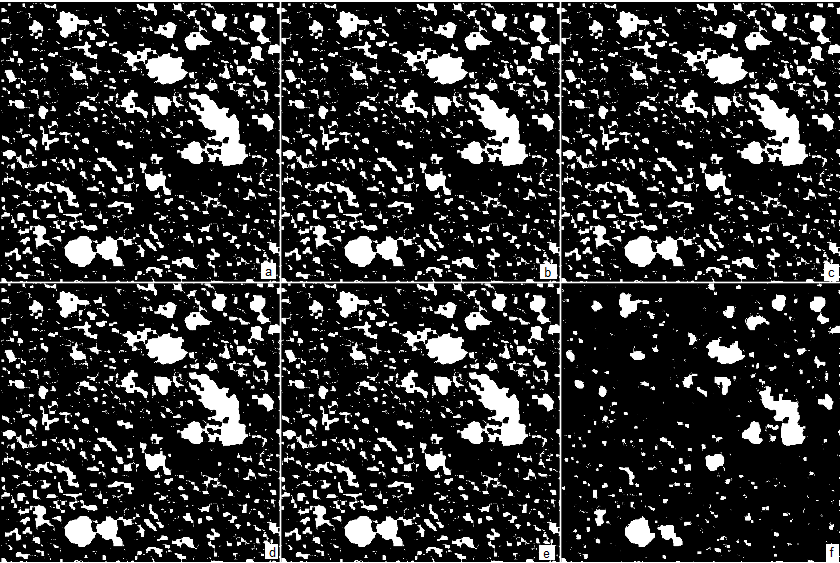
\includegraphics[width=\textwidth]{Imagenes/Resultados script morfologico/GS09-labeled.png}
     %\hfill
     \caption{Resultado del filtrado con topbottom y binarizado con distintos valores de percentil, a) 0,1, b) 1, c) 10, d) 20, e) 50 y f) 90 }
    \label{topbottom}
\end{figure}